% 
% File:     evaluation.tex
% Author:   awl8049
% Revision: 
% 
\chapter{Chaotic Attractor Predictor Evaluation}
\label{chp:evaluation}
Experiments were carried out to evaluate the performance of the CAP
power models built for approximating dynamic system solutions.  The
first experiment aimed to confirm the time complexity of CAP.  Making
use of MATLAB, our CAP code was executed on the two servers specified in
Table~\ref{tab:hardware}.  As the execution times on both servers
provide the same trend, only those collected from the SUN Fire 2200
server (AMD Opteron) are demonstrated here.  The code execution time
results versus $n$ (the number of future observations) is illustrated in
\figurename~\ref{fig:complexity}, where the result curve confirms CAP
time complexity in $O(n^{2})$.  Separately, the CAP execution time as a
function of $p$ (the number of past observations) on the SUN Fire server
is shown in \figurename~\ref{fig:complexityp}, where the time indeed is
linear with respect to $p$, as claimed earlier in our time complexity
subsection.  In practice, a moderate $p$ (of, say, 100) and a small $n$
(of, say, 5) may be chosen under CAP for high accuracy and very low time
complexity in real-time applications.  The results of distant future
(corresponding to a larger $n$) can be predicted by a step-wise process,
with each step predicting the near future outcomes (using $n$ = 5).

\begin{table}[t]
  \centering
  \caption{Server configurations for evaluation}
  \label{tab:hardware}
  \begin{tabular}{l l l}
   \hline
    &\textbf{Sun Fire 2200}&\textbf{Dell PowerEdge R610}\\  
    \hline
    CPU&2 AMD Opteron&2 Intel Xeon (Nehalem) 5500\\
    CPU L2 cache&2x2MB&4MB\\
    Memory&8GB&9GB\\
    Internal disk&2060GB&500GB\\
    Network&2x1000Mbps&1x1000Mbps\\
    Video&On-board&NVIDA Quadro FX4600\\
    Height&1 rack unit&1 rack unit\\
    \hline
  \end{tabular}
\end{table}

\begin{table}[t]
  \centering
  \caption{SPEC CPU2006 benchmarks used for evaluation}
  \label{tab:addspec}
  \begin{tabular}{c c p{5cm}}
    \hline
    \multicolumn{3}{l}{\textbf{Integer Benchmark}} \\
    \hline
    Astar&C++&Path Finding\\
    Gobmk&C&Artificial Intelligence: Go\\
    \multicolumn{3}{l}{\textbf{FP Benchmarks}} \\
    \hline
    Calculix&C++/F90&Structural Mechanics\\
    Zeusmp&F90&Computational Fluid Dynamics\\
    \hline
  \end{tabular}
\end{table}

\section{Evaluation environment}
\label{sec:measurementtools}
The operating system used in our test servers is OpenSolaris (namely,
Solaris 11).  Evaluation results are collected from the system baseboard
controller using the IPMI interface via the OpenSolaris
\texttt{ipmitool} utility.  Processor performance counters are collected
on a system-wide basis by means of \texttt{cpustat}, \texttt{iostat},
and \texttt{ipmitool} utilities in OpenSolaris.  Of these,
\texttt{iostat} and \texttt{ipmitool} are available across all
UNIX-based operating systems commonly employed by data centers, while
\texttt{cpustat} is an OpenSolaris-specific utility (which is being
ported to Linux).

\begin{table}[t]
  \centering
  \caption{Branch and Memory Access Patters of Evaluation Benchmarks}
  \label{tab:benchstats}
\begin{tabular}{lllllrrr}
\hline
% BEGIN RECEIVE ORGTBL perfmetrics
Benchmark & Inst Count & Branches & Loads & Stores \\
 & (Billions) &  &  &  \\
\hline
astar & 1,200 & 15.57\% & 40.34\% & 13.75\% \\
gobmk & 1,603 & 19.51\% & 29.72\% & 15.25\% \\
calculix & 3,041 & 4.11\% & 40.14\% & 9.95\% \\
zeusmp & 1,566 & 4.05\% & 36.22\% & 11.98\% \\
\hline
% END RECEIVE ORGTBL perfmetrics
\end{tabular}
\end{table}
\begin{comment}
#+ORGTBL: SEND perfmetrics orgtbl-to-latex :splice t :skip 0
| Benchmark | Inst Count | Branches | Loads   | Stores  |
|           | (Billions) |          |         |         |
|-----------+------------+----------+---------+---------|
| astar     | 1,200      | 15.57\%  | 40.34\% | 13.75\% |
| gobmk     | 1,603      | 19.51\%  | 29.72\% | 15.25\% |
| calculix  | 3,041      | 4.11\%   | 40.14\% | 9.95\%  |
| zeusmp    | 1,566      | 4.05\%   | 36.22\% | 11.98\% |
|-----------+------------+----------+---------+---------|
\end{comment}

Four benchmarks from the SPEC CPU2006 benchmark suite were used for the
evaluation purpose, as listed in Table~\ref{tab:addspec}), and they are
different from those employed earlier for CAP creation (as listed in
Table V). It is noted that selection of benchmarks for both calibration
and evaluation were selected to sufficiently exercise processor, cache,
and memory again per the decision criteria in \cite{Phansalkar2007},
with the additional criterion of selecting workloads more common to
server environments. As illustrated in Table~\ref{tab:benchstats}
(per results from \cite{Phansalkar2007}), the mix of instructions
exercises the key components of processor, memory, and cache in the
dynamic system which we model with CAP. In addition, the four
benchmarks used in our evaluation represent the type of high-utilization
workloads in server environments per typical industry use of the SPEC
CPU2006 benchmark suite \cite{Cisco2010}.
\begin{table}[]
  \caption{Model errors for CAP (under $n=5$, $p=100$, $r=14$), AR(1),
    MARS, and EWMA on AMD Opteron server}
  \centering
    \label{tab:modelerroropt}
    \begin{tabular}[phtb]{c | r r c | r r c}
      \hline
      \multicolumn{1}{c|}{}&\multicolumn{3}{c|}{\textbf{CAP}}&\multicolumn{3}{c}{\textbf{AR}}\\
      \hline
  &\multicolumn{1}{c}{\textbf{Avg}}&\multicolumn{1}{c}{\textbf{Max}}&\multicolumn{1}{c|}{\textbf{RMSE}}&\multicolumn{1}{c}{\textbf{Avg}}&\multicolumn{1}{c}{\textbf{Max}}&\multicolumn{1}{c}{\textbf{RMSE}}\\
\multicolumn{1}{c|}{\textbf{Benchmark}}&\multicolumn{1}{c}{\textbf{Err \%}}&\multicolumn{1}{c}{\textbf{Err \%}}&\multicolumn{1}{c|}{}&\multicolumn{1}{c}{\textbf{Err \%}}&\multicolumn{1}{c}{\textbf{Err \%}}&\multicolumn{1}{c }{\textbf{}}\\
        \hline
      Astar &0.9\%&5.5\%&0.72&3.1\%&8.9\%&2.26\\
      Games &1.0\%&6.8\%&2.06&2.2\%&9.3\%&2.06\\
      Gobmk &1.6\%&5.9\%&2.30&1.7\%&9.0\%&2.30\\
      Zeusmp&1.0\%&5.6\%&2.14&2.8\%&8.1\%&2.14\\
      \hline
      \multicolumn{1}{c|}{}&\multicolumn{3}{c|}{\textbf{MARS}}&\multicolumn{3}{c}{\textbf{EWMA}}\\
      \hline
  &\multicolumn{1}{c}{\textbf{Avg}}&\multicolumn{1}{c}{\textbf{Max}}&\multicolumn{1}{c|}{\textbf{RMSE}}&\multicolumn{1}{c}{\textbf{Avg}}&\multicolumn{1}{c}{\textbf{Max}}&\multicolumn{1}{c}{\textbf{RMSE}}\\
\multicolumn{1}{c|}{\textbf{Benchmark}}&\multicolumn{1}{c}{\textbf{Err \%}}&\multicolumn{1}{c}{\textbf{Err \%}}&\multicolumn{1}{c|}{}&\multicolumn{1}{c}{\textbf{Err \%}}&\multicolumn{1}{c}{\textbf{Err \%}}&\multicolumn{1}{c }{\textbf{}}\\
      \hline
      Astar &2.5\%&9.3\%&2.12&1.2\%&7.9\%&2.40\\
      Games &3.0\%&9.7\%&2.44&1.1\%&7.8\%&1.42\\
      Gobmk &3.0\%&9.1\%&2.36&1.0\%&6.9\%&2.30\\
      Zeusmp&2.8\%&7.9\%&2.34&1.8\%&9.2\%&2.01\\
      \hline
    \end{tabular}
  \end{table}

The benchmarks were executed on the two servers specified in
Table~\ref{tab:hardware}, with performance metrics gathered during the
course of execution.  Power consumed is measured by a WattsUP power meter
\cite{WattsUp2006a}, connected between the AC Main and the server under
test.  The power meter measures the total and average wattage,
voltage, and amperage over the run of a workload.  The internal memory
of the power meter is cleared at the start of each run and the measures
collected during the runs are downloaded (after execution completion)
from meter's internal memory into a spreadsheet.  Current flow on
different voltage domains in the server is measured using an Agilent
MSO6014A oscilloscope, with one Agilent 1146A current probe per server
power domain (12v, 5v, and 3.3v).  This data was collected from the
oscilloscope at the end of each benchmark execution on a server and then
stored in a spreadsheet on the test host.

\begin{figure}[]
  \centering
  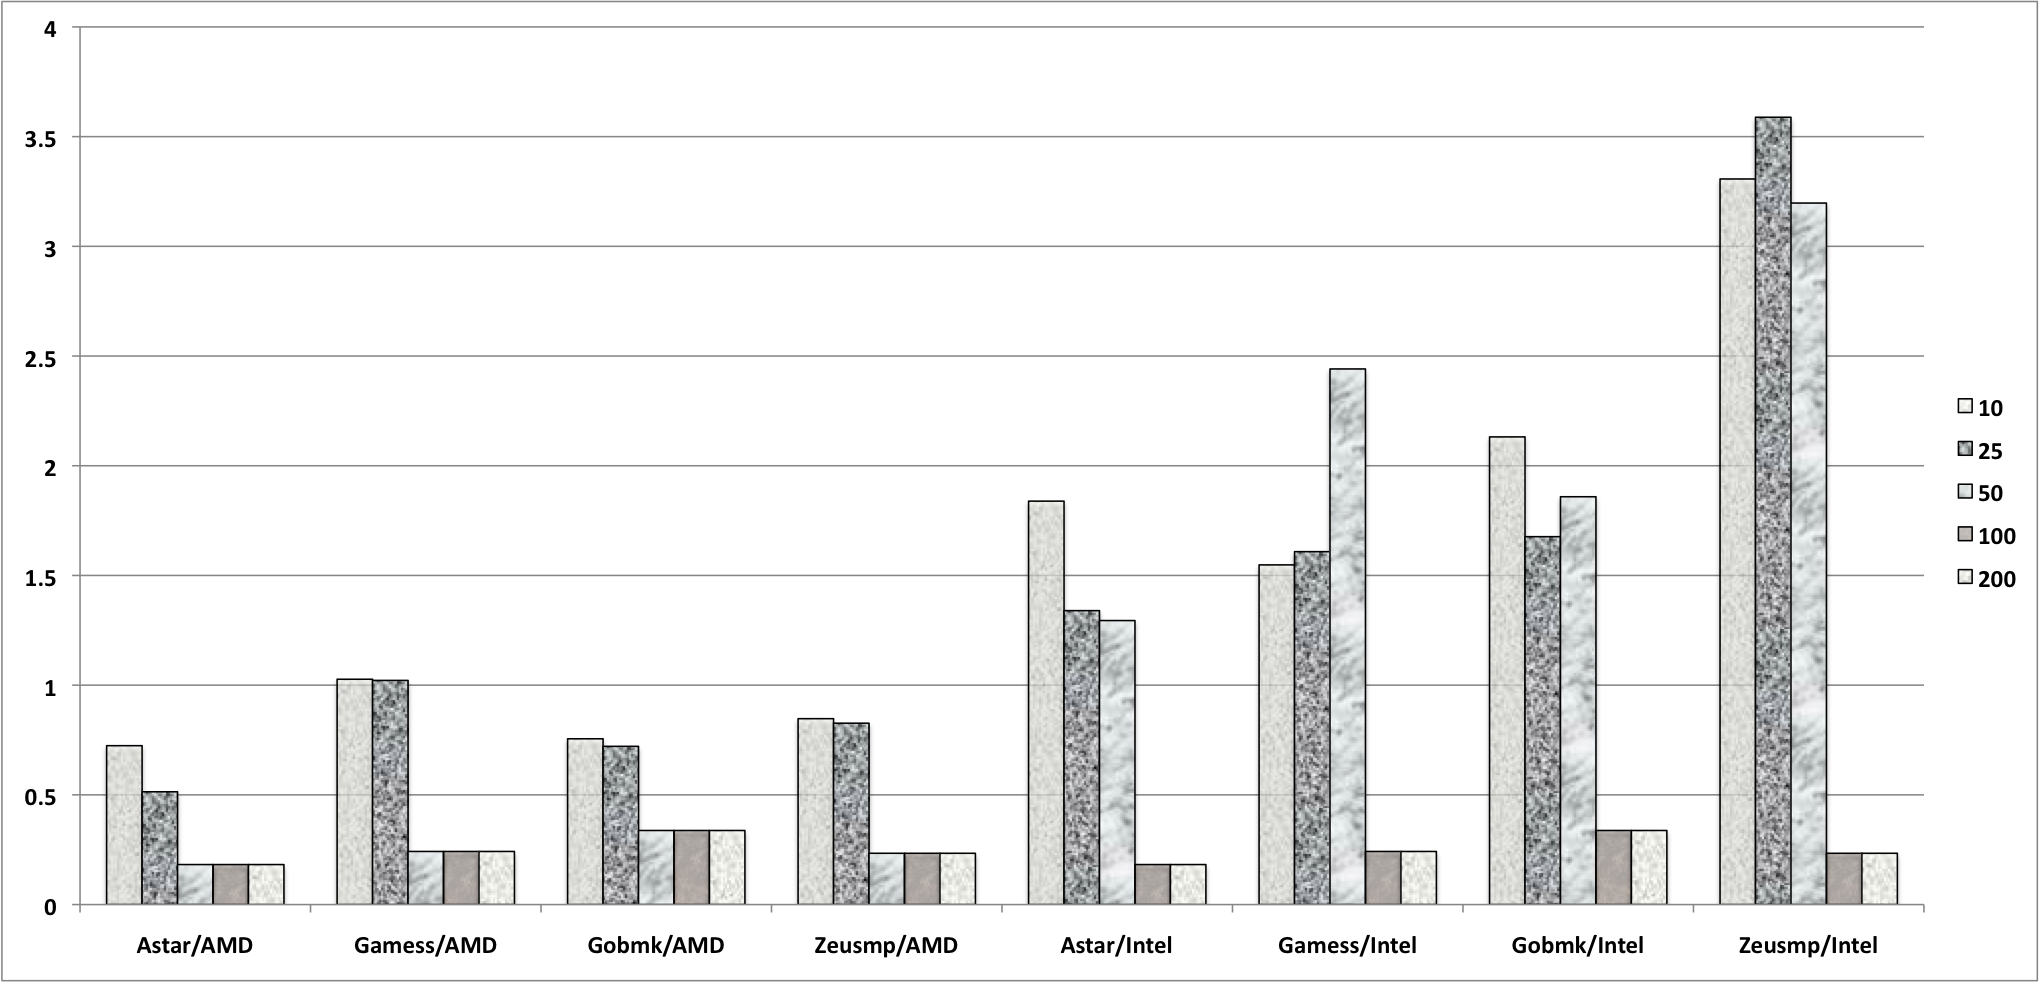
\includegraphics[width=1.0\linewidth,height=2.5in]{rmsep}
  \caption{Root Mean Square Error (RMSE) for different values of $p$.}
  \label{fig:rmsep}
\end{figure}
\section{Results}
\label{sec:htcase}
While the number of measures per observation ($r$) is fixed for a given
server in our evaluation (equal to 14 for the Sun Fire server and to 19
for Dell PowerEdge server), the CAP prediction time and accuracy depend
on $p$ (the number of past observations) and $n$ (the number of future
observations), as stated in Section~\ref{sec:cappcreate}.  In our
evaluation, the CAP prediction error rates of various benchmark codes
for a range of $p$ under a given $n$ were gathered, as demonstrated in
\figurename~\ref{fig:rmsep}, where $n$ equals 5.  It can be seen from
the figure that the error rates are fairly small (and stay almost
unchanged) when $p$ is within 100 to 200, but they rise considerably
when $p$ drops to 50 or below.  In subsequent figures, the prediction
results of CAP include only those for $n = 5$ and $p = 100$.  Each
benchmark was executed to collect the first $p=100$ points on the
attractor, at which point the next $n$=5 points were used to
compute the estimated power for the $t, t+1,\ldots,t+5$ energy estimates
in each time cycle.

\begin{figure}[]
  \centering
  \subfloat[Astar/CAP.]{%
    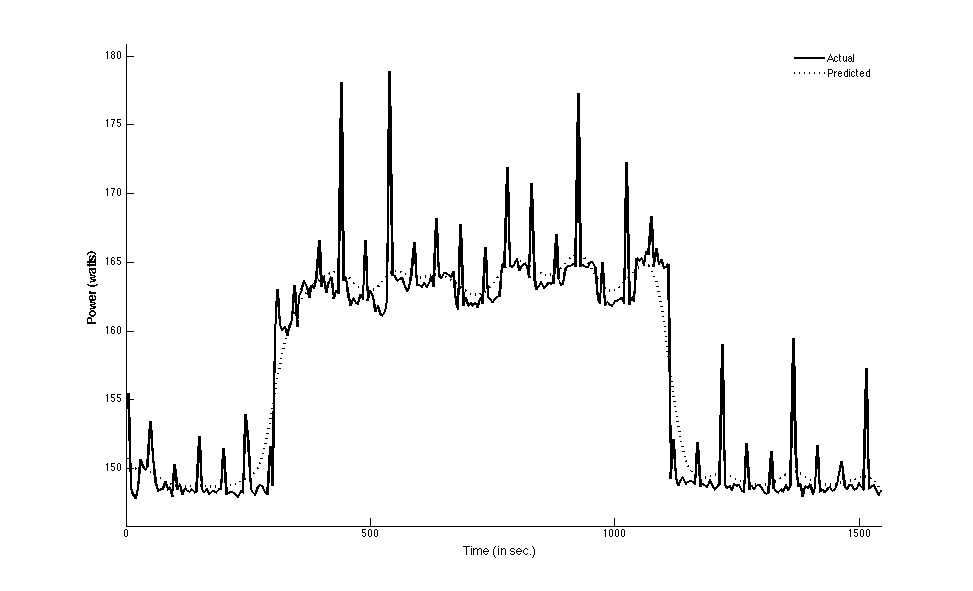
\includegraphics[width=0.5\linewidth,height=2in]{allpower/amd_ch_astar}
  }
  \subfloat[Astar/AR(1)).]{%
    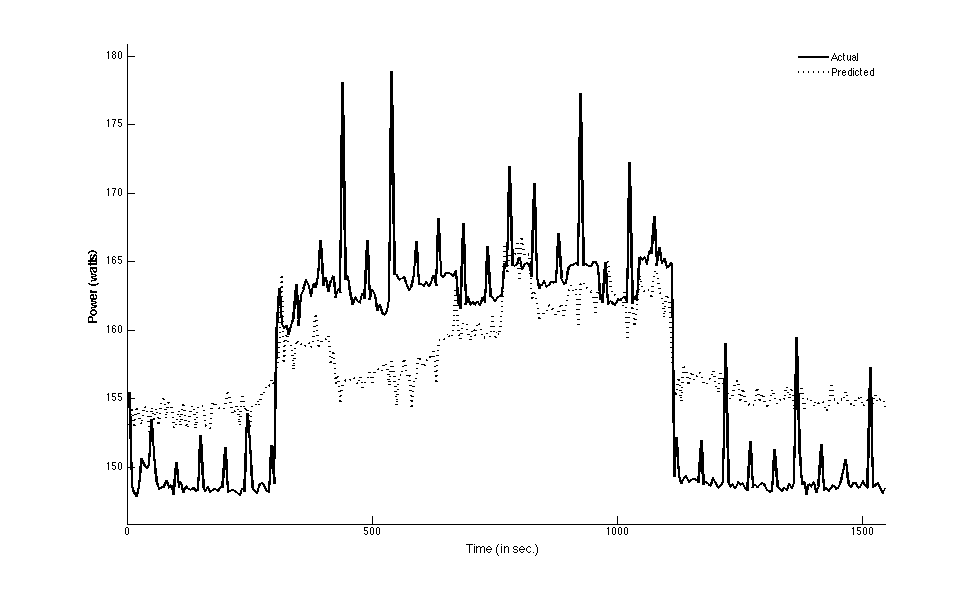
\includegraphics[width=0.5\linewidth,height=2in]{allpower/amd_ar_astar}
  }\\
  \subfloat[Zeusmp/CAP.]{%
    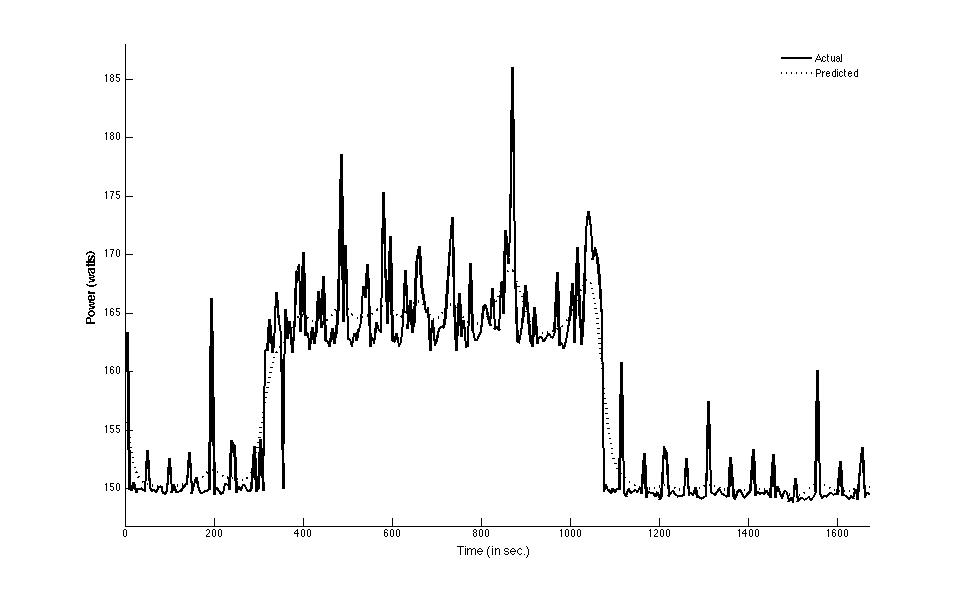
\includegraphics[width=0.5\linewidth,height=2in]{allpower/amd_ch_zeusmp}
  }
  \subfloat[Zeusmp/AR(1).]{%
    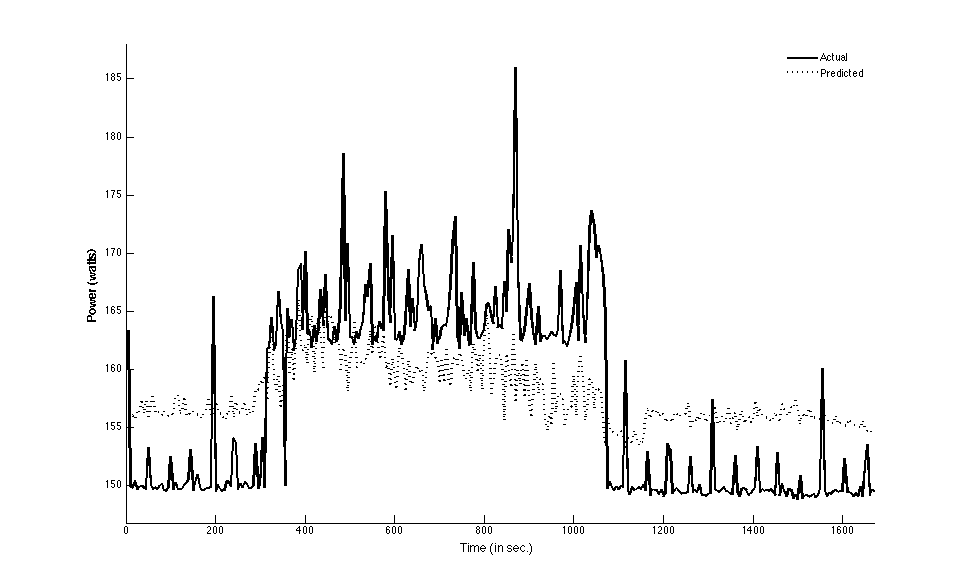
\includegraphics[width=0.5\linewidth,height=2in]{allpower/amd_ar_zeusmp}
  }
  \caption{Actual power results versus predicted results for AMD Opteron.}
  \label{fig:compareamd}
\end{figure}
The predicted power consumption results of CAP during the execution of
Astar and Zeusmp on a HyperTransport-based server are demonstrated in
\figurenames~\ref{fig:compareamd}(a) and \ref{fig:compareamd}(c).  The
predicted values are seen to track closely to the measured readings
(obtained using the WattsUP power meter and indicated by solid curves),
with the error rate ranging between 0.9\% and 1.6\%.  For comparison,
the predicted power consumption outcomes during the execution of same
selected benchmarks under AR(1) are depicted in
\figurenames~\ref{fig:compareamd}(b) and \ref{fig:compareamd}(d).  As
expected, AR(1) exhibits poor outcomes over any given short execution
window, with maximum errors ranging from 7.9\% to 9.3\%, despite that
the prediction error over the whole execution period may be less.  CAP
enjoys much better prediction behavior than its linear regressive
counterpart.

\begin{figure}[]
  \centering
  \subfloat[Astar/CAP.]{%
    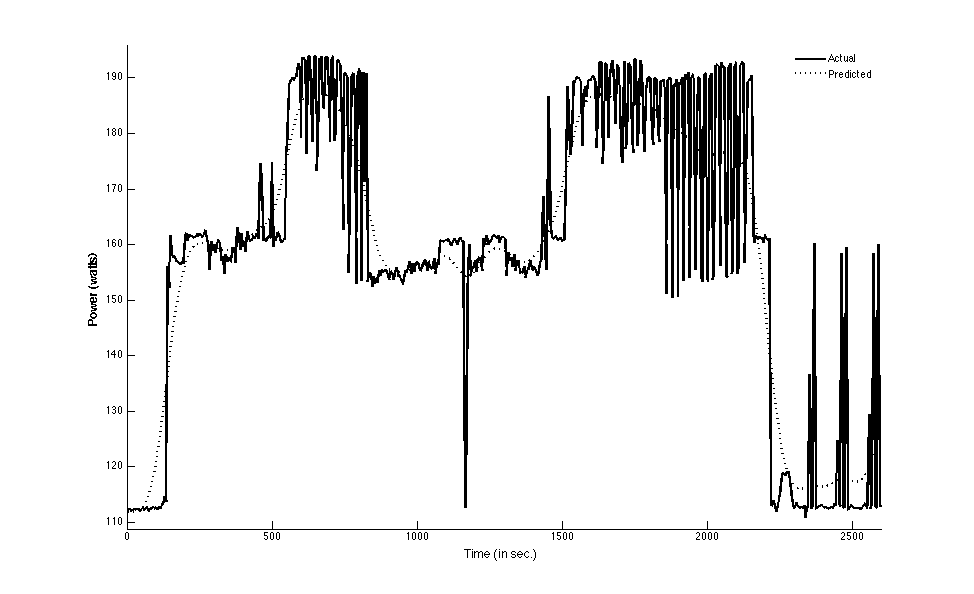
\includegraphics[width=0.5\linewidth,height=2in]{allpower/intel_ch_astar}
  }
  \subfloat[Astar/AR(1)).]{%
    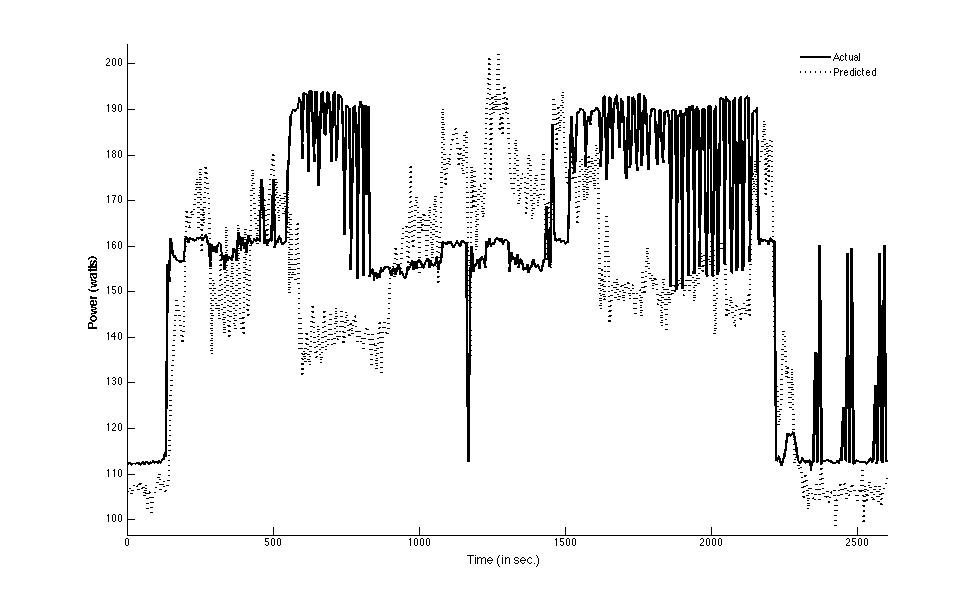
\includegraphics[width=0.5\linewidth,height=2in]{allpower/intel_ar_astar}
  }\\
  \subfloat[Zeusmp/CAP.]{%
    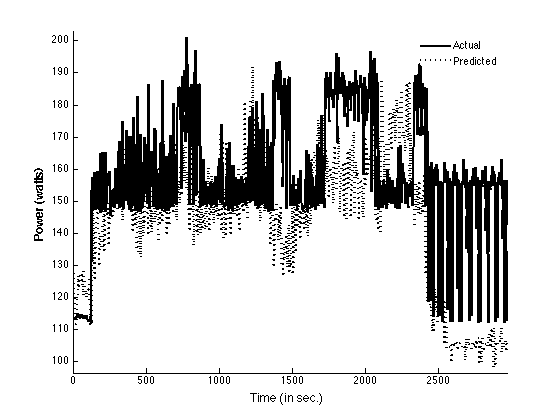
\includegraphics[width=0.5\linewidth,height=2in]{allpower/intel_ch_zeusmp}
  }
  \subfloat[Zeusmp/AR(1).]{%
    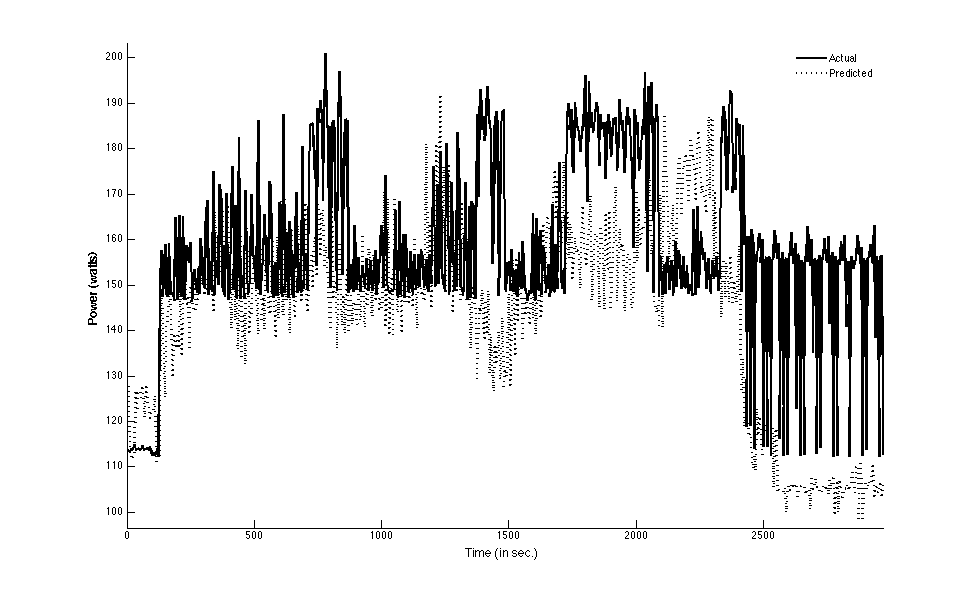
\includegraphics[width=0.5\linewidth,height=2in]{allpower/intel_ar_zeusmp}
  }
  \caption{Actual power results versus predicted results for an Intel
    Nehalem server.}
  \label{fig:compareintel}
\end{figure}
The predicted power consumption results under CAP over the benchmark
execution period for the QPL-based server (Dell PowerEdge) are
demonstrated in \figurenames~\ref{fig:compareintel}(a) and
\ref{fig:compareintel}(c), where the actual power consumption amounts
obtained by the WattsUP meter are shown by solid curves.  Again, CAP is
seen to exhibit impressive performance, tracking the actual amounts
closely, with the error rate ranging between 1.0\% and 3.3\%.  The root
mean square errors for CAP remain within small values.  In contrast,
AR(1) suffers from poor prediction behavior, as can be discovered in
\figurenames~\ref{fig:compareintel}(b) and \ref{fig:compareintel}(d),
where outcomes of same benchmarks executed on the Dell PowerEdge server
are depicted.  It yields the maximum error up to 20.8\% (or 20.6\%) for
the Astar (or Zeusmp) benchmark.  {\addtolength{\tabcolsep}{-3pt}
\begin{table}[]
  \footnotesize
  \caption{Model errors for CAP (under $n=5$, $p=100$, $r=19$), AR, MARS, and
    EWMA predictors on Intel Nehalem server}
  \centering
    \label{tab:modelerroroptIntel}
    \begin{tabular}[phtb]{c | r r c | r r c}
      \hline
      \multicolumn{1}{c|}{}&\multicolumn{3}{c|}{\textbf{CAP}}&\multicolumn{3}{c}{\textbf{AR}}\\
        \hline
  &\multicolumn{1}{c}{\textbf{Avg}}&\multicolumn{1}{c}{\textbf{Max}}&\multicolumn{1}{c|}{\textbf{RMSE}}&\multicolumn{1}{c}{\textbf{Avg}}&\multicolumn{1}{c}{\textbf{Max}}&\multicolumn{1}{c}{\textbf{RMSE}}\\
\multicolumn{1}{c|}{\textbf{Benchmark}}&\multicolumn{1}{c}{\textbf{Err \%}}&\multicolumn{1}{c}{\textbf{Err \%}}&\multicolumn{1}{c|}{}&\multicolumn{1}{c}{\textbf{Err \%}}&\multicolumn{1}{c}{\textbf{Err \%}}&\multicolumn{1}{c }{\textbf{}}\\
      \hline
      Astar &1.1\%&20.8\%&1.83&5.9\%&28.5\%&4.94\\
      Games &1.0\%&14.8\%&1.54&5.6\%&44.3\%&5.54\\
      Gobmk &1.0\%&21.5\%&2.13&5.3\%&27.8\%&4.83\\
      Zeusmp&3.3\%&20.6\%&3.31&7.7\%&31.8\%&7.24\\
      \hline
      \multicolumn{1}{c|}{}&\multicolumn{3}{c|}{\textbf{MARS}}&\multicolumn{3}{c}{\textbf{EWMA}}\\
      \hline
  &\multicolumn{1}{c}{\textbf{Avg}}&\multicolumn{1}{c}{\textbf{Max}}&\multicolumn{1}{c|}{\textbf{RMSE}}&\multicolumn{1}{c}{\textbf{Avg}}&\multicolumn{1}{c}{\textbf{Max}}&\multicolumn{1}{c}{\textbf{RMSE}}\\
\multicolumn{1}{c|}{\textbf{Benchmark}}&\multicolumn{1}{c}{\textbf{Err \%}}&\multicolumn{1}{c}{\textbf{Err \%}}&\multicolumn{1}{c|}{}&\multicolumn{1}{c}{\textbf{Err \%}}&\multicolumn{1}{c}{\textbf{Err \%}}&\multicolumn{1}{c }{\textbf{}}\\
      \hline
      Astar &5.4\%&28.0\%&4.97&3.7\%&32.4\%&2.98\\
      Games &4.7\%&33.0\%&4.58&1.8\%&27.3\%&2.19\\
      Gobmk &4.1\%&27.9\%&4.73&3.9\%&28.4\%&2.73\\
      Zeusmp&11.6\%&32.2\%&8.91&5.0\%&31.3\%&2.81\\
      \hline
    \end{tabular}
  \end{table}
}
\section{Further discussion}
\label{sec:caseanalysis}
Tables~\ref{tab:modelerroropt} (or \ref{tab:modelerroroptIntel})
compares the errors of evaluation benchmarks for the server with the
HyperTransport (or QPL) structure, under four different prediction
mechanisms: CAP, AR, MARS, and EWMA. Large errors exhibited by AR,
MARS, and EWMA overwhelm the advantages gained from their simplicity.
The table results indicate the limitations entailed by using a linear
technique, such as AR time series, to predict dynamic system behavior;
similar issues exist for piecewise and moving average techniques, such as
MARS and EWMA.  Earlier attempts were made to address this issue by
incorporating corrective mechanisms in combination with these
predictors.  An example attempt employed machine learning to monitor 
mis-prediction, with recalibration invoked when required
\cite{Coskun2008}.  CAP eliminates the need for any corrective mechanism
by directly addressing the system dynamics, thereby avoiding wide drifts in
prediction experienced by other prediction techniques.

The model developed in this work is valid for any
dual-core/dual-processor system using NUMA memory access connected in a
point-to-point manner using the HyperTransport or the QPL structures.
However, it can be scaled to quad-core dual processors based on those
two structures.  One would expect to see a slight difference or
variation in power prediction due to a greater or less affect of die
temperatures on the other performance measures.  Under a dual-core
quad-processor server, for example, additional regression variables
would be incorporated in $E_{proc}$, giving rise to more performance
measures (i.e., a larger $r$).  Similarly, more PeCs related to cache
misses would then be involved in $E_{mem}$.  The solution approach of
CAP remains exactly identical, except for a larger $r$ in its prediction
computation.

% Following comment block used by GNU-EMACS and AUCTEX packages
% Please do not remove.
%%% Local Variables: 
%%% mode: latex
%%% TeX-master: "dissertation.tex"
%%% TeX-PDF-mode: t
%%% TeX-source-correlate-mode: t
%%% End: 
